% PopAgent System Walkthrough
% Comprehensive Technical Documentation for Presentation

\documentclass[11pt]{article}

\usepackage[utf8]{inputenc}
\usepackage[T1]{fontenc}
\usepackage{geometry}
\geometry{margin=1in}
\usepackage{hyperref}
\usepackage{booktabs}
\usepackage{amsmath}
\usepackage{amssymb}
\usepackage{graphicx}
\usepackage{xcolor}
\usepackage{listings}
\usepackage{algorithm}
\usepackage{algorithmic}
\usepackage{tcolorbox}
\usepackage{tikz}
\usetikzlibrary{shapes,arrows,positioning,fit,backgrounds,calc,decorations.pathreplacing}
\usepackage{pgfplots}
\pgfplotsset{compat=1.17}

% Custom colors
\definecolor{codeblue}{RGB}{0,102,204}
\definecolor{codegray}{RGB}{128,128,128}
\definecolor{codegreen}{RGB}{0,128,0}
\definecolor{backcolor}{RGB}{245,245,245}
\definecolor{gold}{RGB}{255,215,0}

% Code listing style
\lstset{
    backgroundcolor=\color{backcolor},
    basicstyle=\ttfamily\small,
    keywordstyle=\color{codeblue}\bfseries,
    commentstyle=\color{codegray},
    stringstyle=\color{codegreen},
    breaklines=true,
    frame=single,
    rulecolor=\color{gray},
}

% Custom box for key concepts
\newtcolorbox{keybox}[1][]{
    colback=blue!5,
    colframe=blue!50!black,
    title=#1,
    fonttitle=\bfseries
}

\newtcolorbox{questionbox}[1][]{
    colback=orange!5,
    colframe=orange!50!black,
    title=#1,
    fonttitle=\bfseries
}

\title{\Huge \textbf{PopAgent: System Architecture Walkthrough} \\[0.5em]
\Large Multi-Agent LLM Trading with Adaptive Method Selection}
\author{Technical Documentation for Presentation}
\date{\today}

\begin{document}

\maketitle

\tableofcontents
\newpage

%==============================================================================
\section{Background and Prerequisites}
%==============================================================================

This section provides essential background for readers unfamiliar with the domain.

\subsection{What is Algorithmic Trading?}

\textbf{Algorithmic trading} uses computer programs to make trading decisions automatically. Instead of humans manually deciding when to buy or sell assets, algorithms analyze data and execute trades.

\begin{center}
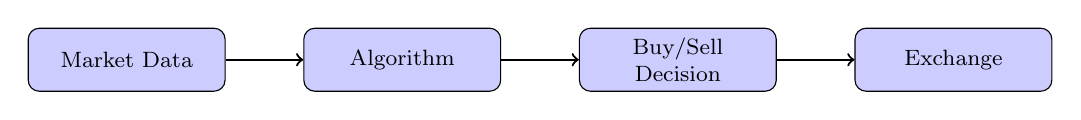
\begin{tikzpicture}[
    box/.style={rectangle, draw, rounded corners, fill=blue!20, minimum width=2.5cm, minimum height=0.8cm, align=center, font=\footnotesize},
    arrow/.style={->, thick}
]
\node[box] (data) at (0, 0) {Market Data};
\node[box] (algo) at (3.5, 0) {Algorithm};
\node[box] (decision) at (7, 0) {Buy/Sell\\Decision};
\node[box] (exchange) at (10.5, 0) {Exchange};

\draw[arrow] (data) -- (algo);
\draw[arrow] (algo) -- (decision);
\draw[arrow] (decision) -- (exchange);
\end{tikzpicture}
\end{center}

\subsection{Key Terms Glossary}

\begin{center}
\begin{tabular}{|l|p{10cm}|}
\hline
\textbf{Term} & \textbf{Definition} \\
\hline
\textbf{LLM} & Large Language Model (e.g., GPT-4, Claude). AI models trained on text that can understand and generate human language. \\
\hline
\textbf{OHLCV} & Open, High, Low, Close, Volume -- the 5 key data points for each time period (candle) in price data. \\
\hline
\textbf{Agent} & An autonomous software component that perceives its environment and takes actions to achieve goals. \\
\hline
\textbf{Multi-Agent System} & Multiple agents working together, each specializing in different tasks. \\
\hline
\textbf{Method} & A specific algorithm or technique (e.g., RSI, ARIMA, Kelly Criterion). \\
\hline
\textbf{Inventory} & The pool of available methods an agent can choose from. \\
\hline
\textbf{Perpetual Futures} & Cryptocurrency derivatives that let traders bet on price movements with leverage, no expiration date. \\
\hline
\textbf{PnL} & Profit and Loss -- how much money was made or lost. \\
\hline
\textbf{Sharpe Ratio} & Risk-adjusted return measure. Higher = better. \\
\hline
\textbf{Drawdown} & Peak-to-trough decline in portfolio value. \\
\hline
\end{tabular}
\end{center}

\subsection{Why is This Problem Hard?}

\begin{enumerate}
    \item \textbf{Non-stationary markets}: What works today may fail tomorrow. Bull markets, bear markets, and sideways markets require different strategies.

    \item \textbf{Limited data}: Unlike games with unlimited simulations, financial data is scarce. We can't just ``play'' millions of episodes.

    \item \textbf{Noisy signals}: Price movements are partly random. Even good strategies lose sometimes.

    \item \textbf{Interpretability requirement}: Traders need to understand \textit{why} the system makes decisions. Black-box neural networks are often rejected.

    \item \textbf{Strategy selection}: With hundreds of possible techniques, choosing which ones to use is itself a hard learning problem.
\end{enumerate}

\subsection{What is a ``Method'' in Our System?}

A \textbf{method} is a specific analytical technique or algorithm. Examples:

\begin{itemize}
    \item \textbf{RSI} (Relative Strength Index): Measures if an asset is overbought or oversold
    \item \textbf{ARIMA}: Statistical model for forecasting time series
    \item \textbf{Kelly Criterion}: Formula for optimal position sizing
    \item \textbf{VaR} (Value at Risk): Estimates worst-case loss
\end{itemize}

PopAgent's innovation: instead of hard-coding which methods to use, agents \textit{learn} which methods work best.

\newpage

%==============================================================================
\section{Executive Summary}
%==============================================================================

\begin{keybox}[What is PopAgent?]
PopAgent is a \textbf{multi-agent trading system} where agents \textbf{learn to SELECT which methods to use} from shared inventories, rather than being locked into fixed strategies. This creates a meta-learning system that discovers optimal method combinations through population-based continual learning.
\end{keybox}

\subsection{The One-Sentence Pitch}

\textit{``Instead of hand-designing trading agents, we let populations of agents learn which analytical methods work best for different market conditions, and share that knowledge across the population.''}

\subsection{Key Innovation}

\begin{center}
\begin{tabular}{|p{6cm}|p{6cm}|}
\hline
\textbf{Traditional Approach} & \textbf{PopAgent Approach} \\
\hline
Fixed agent strategies & Agents SELECT methods dynamically \\
Learn parameters (weights, thresholds) & Learn WHICH methods to use \\
Single best agent & Population discovers combinations \\
Static configurations & Adapts to market conditions \\
\hline
\end{tabular}
\end{center}

\vspace{1em}

% Visual: Traditional vs PopAgent
\begin{figure}[h]
\centering
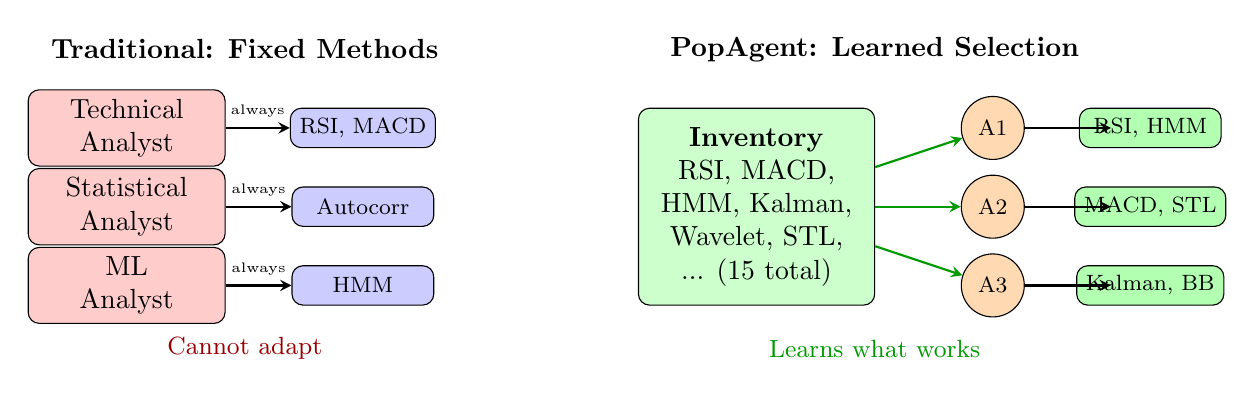
\begin{tikzpicture}[
    box/.style={rectangle, draw, rounded corners, minimum width=2.5cm, minimum height=0.8cm, align=center},
    method/.style={rectangle, draw, fill=blue!20, rounded corners, minimum width=1.8cm, minimum height=0.5cm, font=\footnotesize},
    inv/.style={rectangle, draw, fill=green!20, rounded corners, minimum width=3cm, minimum height=2.5cm, align=center},
    agent/.style={circle, draw, fill=orange!30, minimum size=0.8cm, font=\footnotesize},
    arrow/.style={->, thick, >=stealth}
]

% Traditional side
\node[font=\bfseries] at (-4, 3) {Traditional: Fixed Methods};

\node[box, fill=red!20] (t1) at (-5.5, 2) {Technical\\Analyst};
\node[box, fill=red!20] (t2) at (-5.5, 1) {Statistical\\Analyst};
\node[box, fill=red!20] (t3) at (-5.5, 0) {ML\\Analyst};

\node[method] (m1) at (-2.5, 2) {RSI, MACD};
\node[method] (m2) at (-2.5, 1) {Autocorr};
\node[method] (m3) at (-2.5, 0) {HMM};

\draw[arrow] (t1) -- node[above, font=\tiny] {always} (m1);
\draw[arrow] (t2) -- node[above, font=\tiny] {always} (m2);
\draw[arrow] (t3) -- node[above, font=\tiny] {always} (m3);

% PopAgent side
\node[font=\bfseries] at (4, 3) {PopAgent: Learned Selection};

\node[inv] (inventory) at (2.5, 1) {\textbf{Inventory}\\RSI, MACD,\\HMM, Kalman,\\Wavelet, STL,\\... (15 total)};

\node[agent] (a1) at (5.5, 2) {A1};
\node[agent] (a2) at (5.5, 1) {A2};
\node[agent] (a3) at (5.5, 0) {A3};

\draw[arrow, color=green!60!black] (inventory) -- (a1);
\draw[arrow, color=green!60!black] (inventory) -- (a2);
\draw[arrow, color=green!60!black] (inventory) -- (a3);

\node[method, fill=green!30] at (7.5, 2) {RSI, HMM};
\node[method, fill=green!30] at (7.5, 1) {MACD, STL};
\node[method, fill=green!30] at (7.5, 0) {Kalman, BB};

\draw[arrow] (a1) -- (7, 2);
\draw[arrow] (a2) -- (7, 1);
\draw[arrow] (a3) -- (7, 0);

% Labels
\node[font=\small, color=red!60!black] at (-4, -0.8) {Cannot adapt};
\node[font=\small, color=green!60!black] at (4, -0.8) {Learns what works};

\end{tikzpicture}
\caption{Traditional fixed-method agents vs. PopAgent's adaptive method selection}
\label{fig:innovation}
\end{figure}

%==============================================================================
\section{Motivation: Why Build This System?}
%==============================================================================

\subsection{The Problem with Existing Approaches}

\begin{center}
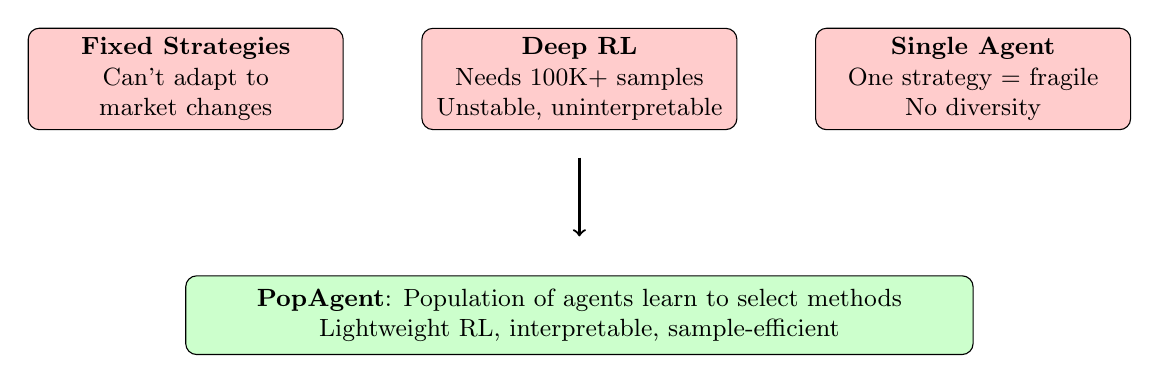
\begin{tikzpicture}[
    problem/.style={rectangle, draw, fill=red!20, rounded corners, minimum width=4cm, minimum height=1cm, align=center, font=\small},
    solution/.style={rectangle, draw, fill=green!20, rounded corners, minimum width=4cm, minimum height=1cm, align=center, font=\small}
]

% Problems
\node[problem] at (0, 4) {\textbf{Fixed Strategies}\\Can't adapt to\\market changes};
\node[problem] at (5, 4) {\textbf{Deep RL}\\Needs 100K+ samples\\Unstable, uninterpretable};
\node[problem] at (10, 4) {\textbf{Single Agent}\\One strategy = fragile\\No diversity};

% Arrow
\draw[->, thick] (5, 3) -- (5, 2);

% Solution
\node[solution, minimum width=10cm] at (5, 1) {\textbf{PopAgent}: Population of agents learn to select methods\\Lightweight RL, interpretable, sample-efficient};

\end{tikzpicture}
\end{center}

\subsection{Research Questions We Address}

\begin{enumerate}
    \item \textbf{RQ1}: Can agents learn \textit{which methods to use} rather than just tuning parameters?

    \item \textbf{RQ2}: Can population-based exploration discover effective method combinations?

    \item \textbf{RQ3}: Can lightweight RL techniques (bandits) match deep RL performance with 100$\times$ fewer samples?

    \item \textbf{RQ4}: Can knowledge transfer accelerate learning without collapsing diversity?
\end{enumerate}

\subsection{Our Contribution}

\begin{keybox}[PopAgent Contributions]
\begin{enumerate}
    \item \textbf{Method Selection Framework}: First system where agents learn \textit{what} to use, not just parameters
    \item \textbf{Population-Based Exploration}: 20 agents explore the combinatorial space of method selections
    \item \textbf{Lightweight RL}: Thompson Sampling + Contextual Baselines + Multi-Step Returns
    \item \textbf{Interpretable Preferences}: Clear, inspectable method preferences (no black boxes)
\end{enumerate}
\end{keybox}

%==============================================================================
\section{System Overview}
%==============================================================================

\subsection{High-Level Architecture}

The system consists of four main layers:

\begin{enumerate}
    \item \textbf{Data Pipeline}: Fetches and processes price data (5 cryptocurrencies) and news
    \item \textbf{Agent Populations}: 4 roles $\times$ 5 agents each = 20 agents total
    \item \textbf{Learning Engine}: Thompson Sampling + Contextual Baselines + Multi-Step Returns
    \item \textbf{Execution}: Paper trading via Bybit Testnet
\end{enumerate}

\subsection{The Trading Pipeline}

Each trading iteration follows this flow:

\begin{figure}[h]
\centering
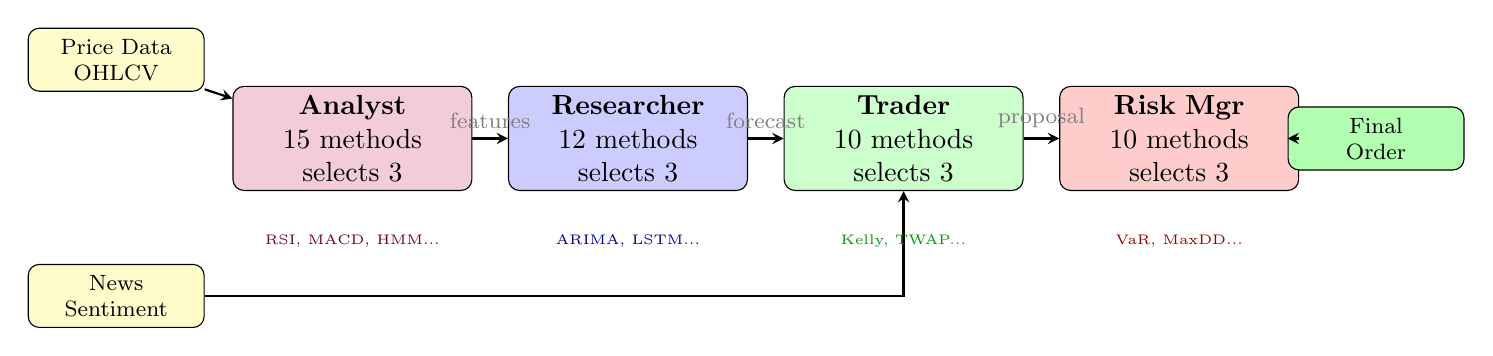
\begin{tikzpicture}[node distance=1.8cm, auto,
    block/.style={rectangle, draw, fill=blue!20, text width=2.8cm, text centered, rounded corners, minimum height=1.2cm},
    data/.style={rectangle, draw, fill=yellow!20, text width=2cm, text centered, rounded corners, minimum height=0.8cm, font=\footnotesize},
    arrow/.style={->, thick, >=stealth},
    label/.style={font=\footnotesize, color=gray}]

    % Data inputs
    \node[data] (price) at (-2, 2) {Price Data\\OHLCV};
    \node[data] (news) at (-2, -1) {News\\Sentiment};

    % Pipeline
    \node[block, fill=purple!20] (analyst) at (1, 1) {\textbf{Analyst}\\15 methods\\selects 3};
    \node[block, fill=blue!20] (researcher) at (4.5, 1) {\textbf{Researcher}\\12 methods\\selects 3};
    \node[block, fill=green!20] (trader) at (8, 1) {\textbf{Trader}\\10 methods\\selects 3};
    \node[block, fill=red!20] (risk) at (11.5, 1) {\textbf{Risk Mgr}\\10 methods\\selects 3};

    % Output
    \node[data, fill=green!30] (order) at (14, 1) {Final\\Order};

    % Arrows with labels
    \draw[arrow] (price) -- (analyst);
    \draw[arrow] (analyst) -- node[above, label] {features} (researcher);
    \draw[arrow] (researcher) -- node[above, label] {forecast} (trader);
    \draw[arrow] (news) -| (trader);
    \draw[arrow] (trader) -- node[above, label] {proposal} (risk);
    \draw[arrow] (risk) -- (order);

    % Inventory indicators
    \node[font=\tiny, color=purple!60!black] at (1, -0.3) {RSI, MACD, HMM...};
    \node[font=\tiny, color=blue!60!black] at (4.5, -0.3) {ARIMA, LSTM...};
    \node[font=\tiny, color=green!60!black] at (8, -0.3) {Kelly, TWAP...};
    \node[font=\tiny, color=red!60!black] at (11.5, -0.3) {VaR, MaxDD...};

\end{tikzpicture}
\caption{The four-stage trading pipeline. Each agent selects 3 methods from its inventory.}
\label{fig:pipeline}
\end{figure}

\textbf{Key insight}: Each role has an \textit{inventory} of methods (10-15), but each agent only \textit{selects 3} at a time. This creates selection pressure.

% Selection pressure visualization
\begin{figure}[h]
\centering
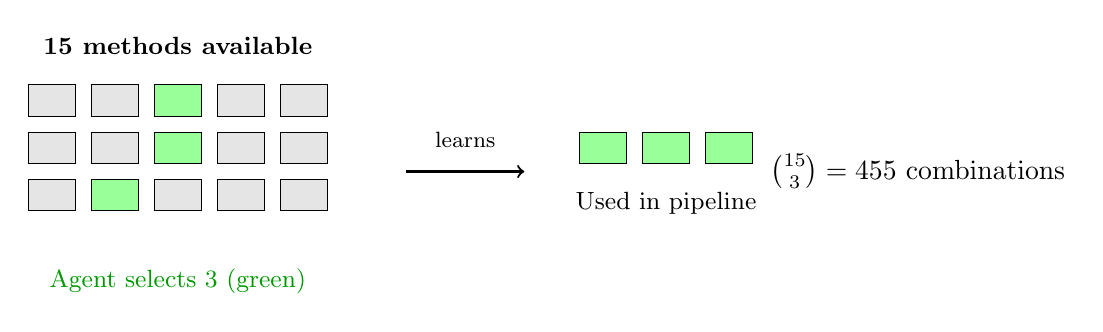
\begin{tikzpicture}[
    method/.style={rectangle, draw, fill=gray!20, minimum width=0.6cm, minimum height=0.4cm, font=\tiny},
    selected/.style={rectangle, draw, fill=green!40, minimum width=0.6cm, minimum height=0.4cm, font=\tiny},
]

% Inventory grid
\foreach \i in {0,...,14} {
    \pgfmathsetmacro{\x}{mod(\i, 5) * 0.8}
    \pgfmathsetmacro{\y}{-floor(\i / 5) * 0.6}
    \ifnum\i=2
        \node[selected] at (\x, \y) {};
    \else\ifnum\i=7
        \node[selected] at (\x, \y) {};
    \else\ifnum\i=11
        \node[selected] at (\x, \y) {};
    \else
        \node[method] at (\x, \y) {};
    \fi\fi\fi
}

\node[font=\small] at (1.6, 0.7) {\textbf{15 methods available}};
\node[font=\small, color=green!60!black] at (1.6, -2.3) {Agent selects 3 (green)};

% Arrow
\draw[->, thick] (4.5, -0.9) -- (6, -0.9);
\node at (5.25, -0.5) {\footnotesize learns};

% Result
\node[selected] at (7, -0.6) {};
\node[selected] at (7.8, -0.6) {};
\node[selected] at (8.6, -0.6) {};

\node[font=\small] at (7.8, -1.3) {Used in pipeline};

% Math
\node at (11, -0.9) {$\binom{15}{3} = 455$ combinations};

\end{tikzpicture}
\caption{Selection pressure: 15 methods, only 3 selected. Creates 455 possible combinations to explore.}
\label{fig:selection_pressure}
\end{figure}

%==============================================================================
\section{The Four Agent Roles}
%==============================================================================

\subsection{Role 1: Analyst (Feature Engineering)}

\begin{keybox}[Analyst's Job]
Transform raw price data into meaningful features that signal trading opportunities.
\end{keybox}

\textbf{Input}: OHLCV price data (Open, High, Low, Close, Volume)

\textbf{Output}: Feature DataFrame with computed indicators

\textbf{Method Inventory (15 methods)}:

\begin{center}
\begin{tabular}{|l|l|p{6cm}|}
\hline
\textbf{Category} & \textbf{Methods} & \textbf{What They Compute} \\
\hline
Technical & RSI, MACD, Bollinger, ADX, Stochastic & Momentum, trend, volatility bands \\
Statistical & Autocorrelation, VolatilityClustering, MeanReversion, Cointegration & Statistical patterns \\
Decomposition & STL, Wavelet, Fourier & Time series decomposition \\
ML-Based & HMM\_Regime, Kalman, IsolationForest & Regime detection, filtering, anomalies \\
\hline
\end{tabular}
\end{center}

\textbf{Example}: An analyst might select \texttt{[RSI, HMM\_Regime, Wavelet]} based on learned preferences.

\subsection{Role 2: Researcher (Forecasting)}

\begin{keybox}[Researcher's Job]
Generate price forecasts with uncertainty quantification.
\end{keybox}

\textbf{Input}: Features from Analyst + historical prices

\textbf{Output}: Point forecast + confidence intervals

\textbf{Method Inventory (12 methods)}:

\begin{center}
\begin{tabular}{|l|l|p{6cm}|}
\hline
\textbf{Category} & \textbf{Methods} & \textbf{What They Do} \\
\hline
Statistical & ARIMA, ExpSmoothing, VAR, GARCH & Classical time series models \\
ML & RandomForest, GradientBoosting, LSTM, TemporalFusion & Machine learning forecasters \\
Uncertainty & Bootstrap, QuantileRegression, Bayesian, Conformal & Confidence interval methods \\
\hline
\end{tabular}
\end{center}

\textbf{Critical Output}: Not just a point forecast, but uncertainty bounds:
\begin{equation}
    \text{Forecast}: \hat{y}_{t+1} = 42{,}150 \pm 320 \text{ (95\% CI)}
\end{equation}

\subsection{Role 3: Trader (Order Generation)}

\begin{keybox}[Trader's Job]
Convert forecasts into concrete trading orders.
\end{keybox}

\textbf{Input}: Forecast + uncertainty from Researcher + news sentiment

\textbf{Output}: Trading order (direction, size, entry price, stop loss, take profit)

\textbf{Method Inventory (10 methods)}:

\begin{center}
\begin{tabular}{|l|l|p{6cm}|}
\hline
\textbf{Category} & \textbf{Methods} & \textbf{What They Control} \\
\hline
Execution & AggressiveMarket, PassiveLimit, TWAP, VWAP & How to execute (speed vs. cost) \\
Sizing & KellyCriterion, FixedFractional, VolatilityScaled & How much to trade \\
Entry & MomentumEntry, ContrarianEntry, BreakoutEntry & When to enter \\
\hline
\end{tabular}
\end{center}

\textbf{Example Order}:
\begin{lstlisting}
{
  "symbol": "BTCUSD.PERP",
  "side": "LONG",
  "position_size": 0.15,
  "leverage": 3,
  "entry_price": 42150,
  "stop_loss": 41500,
  "take_profit": 43200
}
\end{lstlisting}

\subsection{Role 4: Risk Manager (Validation)}

\begin{keybox}[Risk Manager's Job]
Validate orders against risk limits. Can PASS, SOFT\_FAIL (adjust), or HARD\_FAIL (block).
\end{keybox}

\textbf{Input}: Proposed order from Trader

\textbf{Output}: Verdict (PASS / SOFT\_FAIL / HARD\_FAIL) + adjusted order if needed

\textbf{Method Inventory (10 methods)}:

\begin{center}
\begin{tabular}{|l|l|p{6cm}|}
\hline
\textbf{Category} & \textbf{Methods} & \textbf{What They Check} \\
\hline
Position Limits & MaxLeverage, MaxPosition, Concentration & Size constraints \\
Loss Limits & MaxDrawdown, DailyStopLoss, TrailingStop & Loss protection \\
Risk Metrics & VaR, ExpectedShortfall & Statistical risk measures \\
Dynamic & VolatilityAdjusted, RegimeAware & Adaptive limits \\
\hline
\end{tabular}
\end{center}

\textbf{Verdict Logic}:
\begin{itemize}
    \item \textbf{PASS}: Order is within all limits, execute as-is
    \item \textbf{SOFT\_FAIL}: Order violates soft limits, adjust (reduce size/leverage)
    \item \textbf{HARD\_FAIL}: Order violates critical limits, block entirely
\end{itemize}

%==============================================================================
\section{The Method Selection System}
%==============================================================================

This is the \textbf{core innovation} of PopAgent.

\subsection{The Problem with Fixed Strategies}

Traditional approach:
\begin{lstlisting}[language=Python]
class TechnicalAnalyst:
    def analyze(self, prices):
        rsi = compute_rsi(prices)      # Always uses RSI
        macd = compute_macd(prices)    # Always uses MACD
        return rsi, macd               # Fixed methods
\end{lstlisting}

\textbf{Problem}: What if RSI works well in trending markets but poorly in ranging markets? The agent can't adapt.

\subsection{PopAgent's Solution: Method Selection}

Our approach:
\begin{lstlisting}[language=Python]
class MethodSelector:
    inventory = [RSI, MACD, Bollinger, HMM, Kalman, ...]  # 15 options
    preferences = {RSI: 0.8, MACD: 0.3, HMM: 1.2, ...}    # Learned

    def select_methods(self, context):
        # Sample from Beta distributions (Thompson Sampling)
        scores = {m: sample_beta(alpha[m], beta[m]) for m in inventory}
        selected = top_3(scores)  # Pick 3 methods
        return selected           # e.g., [RSI, HMM, Kalman]
\end{lstlisting}

\textbf{Key insight}: The agent learns WHICH methods to use, not just how to tune parameters.

\subsection{Why Inventory > Selection Creates Learning}

\begin{center}
\begin{tabular}{|c|c|c|}
\hline
\textbf{Inventory Size} & \textbf{Selection Size} & \textbf{Possible Combinations} \\
\hline
15 methods & 3 selected & $\binom{15}{3} = 455$ combinations \\
\hline
\end{tabular}
\end{center}

With 455 possible method combinations per role, agents must \textit{learn} which ones work. This is fundamentally different from parameter tuning.

%==============================================================================
\section{Inventory Implementation: Pools and Methods}
%==============================================================================

This section provides the technical details of how methods are stored, registered, and accessed in the PopAgent codebase.

\subsection{The Central Registry Data Structure}

All methods are stored in a single nested dictionary structure:

\begin{lstlisting}[language=Python]
from collections import defaultdict
from typing import Dict, Type

REGISTRY: Dict[str, Dict[str, type]] = defaultdict(dict)
\end{lstlisting}

\begin{keybox}[Registry Structure]
The \texttt{REGISTRY} is a two-level dictionary:
\begin{itemize}
    \item \textbf{Outer key}: Pool name (e.g., \texttt{"analyst.features"}, \texttt{"researcher.forecasting"})
    \item \textbf{Inner key}: Method name (e.g., \texttt{"talib\_stack"}, \texttt{"arima\_x"})
    \item \textbf{Value}: The Python class implementing the method
\end{itemize}
\end{keybox}

\textbf{Visual representation of the registry}:

\begin{figure}[h]
\centering
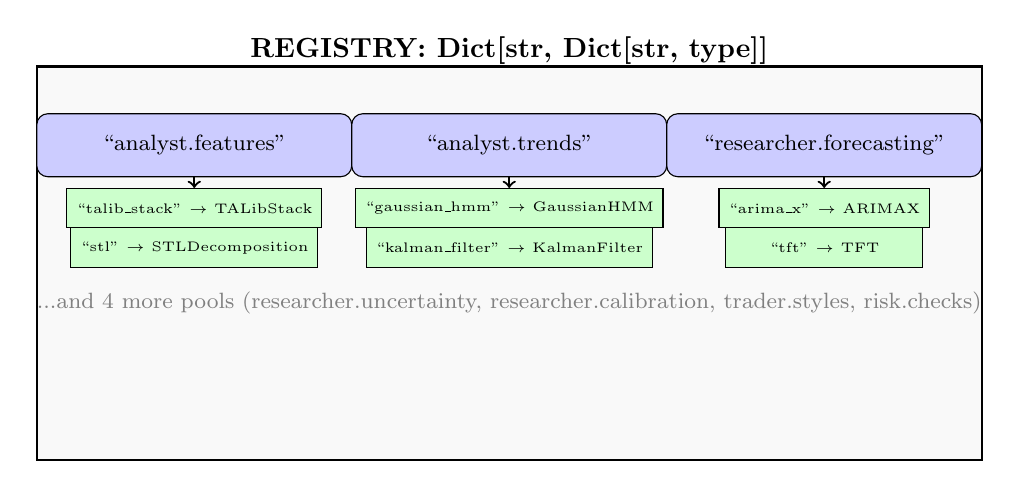
\begin{tikzpicture}[
    pool/.style={rectangle, draw, rounded corners, fill=blue!20, minimum width=4cm, minimum height=0.8cm, align=center, font=\footnotesize},
    method/.style={rectangle, draw, fill=green!20, minimum width=2.5cm, minimum height=0.5cm, font=\tiny},
    arrow/.style={->, thick}
]

% Registry box
\node[rectangle, draw, thick, minimum width=12cm, minimum height=5cm, fill=gray!5] at (0, 0) {};
\node[font=\bfseries] at (0, 2.7) {REGISTRY: Dict[str, Dict[str, type]]};

% Pool 1: analyst.features
\node[pool] (p1) at (-4, 1.5) {``analyst.features''};
\node[method] (m1a) at (-4, 0.7) {``talib\_stack'' $\rightarrow$ TALibStack};
\node[method] (m1b) at (-4, 0.2) {``stl'' $\rightarrow$ STLDecomposition};

% Pool 2: analyst.trends
\node[pool] (p2) at (0, 1.5) {``analyst.trends''};
\node[method] (m2a) at (0, 0.7) {``gaussian\_hmm'' $\rightarrow$ GaussianHMM};
\node[method] (m2b) at (0, 0.2) {``kalman\_filter'' $\rightarrow$ KalmanFilter};

% Pool 3: researcher.forecasting
\node[pool] (p3) at (4, 1.5) {``researcher.forecasting''};
\node[method] (m3a) at (4, 0.7) {``arima\_x'' $\rightarrow$ ARIMAX};
\node[method] (m3b) at (4, 0.2) {``tft'' $\rightarrow$ TFT};

% More pools indicator
\node[font=\footnotesize, color=gray] at (0, -0.5) {...and 4 more pools (researcher.uncertainty, researcher.calibration, trader.styles, risk.checks)};

% Access arrows
\draw[arrow, dashed] (-4, 1.1) -- (m1a);
\draw[arrow, dashed] (0, 1.1) -- (m2a);
\draw[arrow, dashed] (4, 1.1) -- (m3a);

\end{tikzpicture}
\caption{The REGISTRY stores methods organized by pool name, with each pool containing named method classes.}
\label{fig:registry}
\end{figure}

\subsection{The Registration Pattern}

Methods are registered using a Python decorator:

\begin{lstlisting}[language=Python]
def register(pool: str, name: str):
    """Decorator to register an inventory method."""
    def decorator(cls: Type):
        REGISTRY[pool][name] = cls
        cls.pool = pool      # Attach metadata
        cls.name = name
        return cls
    return decorator
\end{lstlisting}

\textbf{Example usage}:

\begin{lstlisting}[language=Python]
@register("analyst.features", "talib_stack")
class TALibStack(FeatureMethod):
    """Technical analysis feature stack using pandas."""
    name = "talib_stack"

    def run(self, price_df: pd.DataFrame, **kwargs) -> pd.DataFrame:
        # Compute EMA, RSI, ATR indicators...
        return features_df
\end{lstlisting}

When Python loads the module, the \texttt{@register} decorator automatically adds the class to the registry.

\subsection{Abstract Interfaces}

Each method type inherits from an abstract base class that defines the expected interface:

\begin{lstlisting}[language=Python]
from abc import ABC, abstractmethod

# ============= Analyst Methods =============
class FeatureMethod(ABC):
    """Base class for feature construction methods."""
    @abstractmethod
    def run(self, price_df: pd.DataFrame, **kwargs) -> pd.DataFrame:
        """Returns DataFrame with computed features."""
        ...

class TrendMethod(ABC):
    """Base class for trend detection methods."""
    @abstractmethod
    def run(self, price_df: pd.DataFrame, **kwargs) -> pd.DataFrame:
        """Returns DataFrame with prob_up, prob_down, regime, slope."""
        ...

# ============= Researcher Methods =============
class ForecastMethod(ABC):
    """Base class for forecasting methods."""
    @abstractmethod
    def run(self, features, trend, **kwargs) -> Dict[str, float]:
        """Returns dict mapping horizon to predicted % change."""
        ...

class UncertaintyMethod(ABC):
    """Base class for uncertainty quantification."""
    @abstractmethod
    def run(self, features, trend, forecast, **kwargs) -> Dict[str, float]:
        """Returns uncertainty metrics (q05, q95, etc.)."""
        ...

class CalibrationMethod(ABC):
    """Base class for probability calibration."""
    @abstractmethod
    def run(self, forecast, **kwargs) -> Dict[str, float]:
        """Returns calibrated forecast dict."""
        ...

# ============= Trader Methods =============
class ExecutionStyleMethod(ABC):
    """Base class for execution style selection."""
    @abstractmethod
    def choose(self, research_summary, news, **kwargs) -> str:
        """Returns execution style name."""
        ...

# ============= Risk Methods =============
class RiskCheckMethod(ABC):
    """Base class for risk validation."""
    @abstractmethod
    def evaluate(self, execution, context) -> Dict[str, Any]:
        """Returns verdict (pass/soft_fail/hard_fail) + envelope."""
        ...
\end{lstlisting}

\subsection{Accessing Methods from the Registry}

Three primary functions for working with the registry:

\begin{lstlisting}[language=Python]
def get(pool: str, name: str) -> Type:
    """Get a registered method class by pool and name."""
    if pool not in REGISTRY:
        raise KeyError(f"Unknown pool: {pool}")
    if name not in REGISTRY[pool]:
        raise KeyError(f"Unknown method '{name}' in pool '{pool}'")
    return REGISTRY[pool][name]

def list_methods(pool: str) -> List[str]:
    """List all registered methods in a pool."""
    return list(REGISTRY[pool].keys())

def list_pools() -> List[str]:
    """List all registered pools."""
    return list(REGISTRY.keys())
\end{lstlisting}

\textbf{Usage examples}:

\begin{lstlisting}[language=Python]
from trading_agents.inventory import get, list_methods, load_all_methods

# First, ensure all methods are loaded
load_all_methods()

# Get a specific method class
TALibStack = get("analyst.features", "talib_stack")
method_instance = TALibStack()
features = method_instance.run(price_df)

# List all methods in a pool
print(list_methods("analyst.features"))
# Output: ['talib_stack', 'stl']

# List all pools
print(list_pools())
# Output: ['analyst.features', 'analyst.trends',
#          'researcher.forecasting', ...]
\end{lstlisting}

\subsection{Dynamic Method Loading}

Methods are loaded dynamically at startup using Python's \texttt{pkgutil}:

\begin{lstlisting}[language=Python]
import pkgutil
import importlib
from pathlib import Path

def load_all_methods() -> None:
    """Import all inventory modules so @register decorators run."""
    pkg_path = Path(__file__).parent

    for finder, name, ispkg in pkgutil.iter_modules([str(pkg_path)]):
        if name.startswith("_"):
            continue
        if ispkg:
            # Load sub-package modules (analyst/, researcher/, etc.)
            subpkg_path = pkg_path / name
            for _, subname, _ in pkgutil.iter_modules([str(subpkg_path)]):
                if not subname.startswith("_"):
                    importlib.import_module(f".{name}.{subname}",
                                           package=__name__)
        else:
            importlib.import_module(f".{name}", package=__name__)
\end{lstlisting}

This pattern allows adding new methods simply by:
\begin{enumerate}
    \item Creating a new Python file in the appropriate subdirectory
    \item Defining a class with the \texttt{@register} decorator
    \item The method is automatically available at next startup
\end{enumerate}

\subsection{Complete Inventory Pools Reference}

\begin{table}[h]
\centering
\footnotesize
\caption{All inventory pools with their registered methods.}
\begin{tabular}{|l|l|l|p{6cm}|}
\hline
\textbf{Pool Name} & \textbf{Interface} & \textbf{Methods} & \textbf{Output} \\
\hline
\texttt{analyst.features} & \texttt{FeatureMethod} & \texttt{talib\_stack}, \texttt{stl} & DataFrame with computed indicators \\
\hline
\texttt{analyst.trends} & \texttt{TrendMethod} & \texttt{gaussian\_hmm}, \texttt{kalman\_filter} & DataFrame with prob\_up, prob\_down, regime, slope \\
\hline
\texttt{researcher.forecasting} & \texttt{ForecastMethod} & \texttt{arima\_x}, \texttt{tft} & Dict mapping horizon to \% change \\
\hline
\texttt{researcher.uncertainty} & \texttt{UncertaintyMethod} & \texttt{bootstrap\_ensemble}, \texttt{quantile\_regression} & Dict with quantiles (q05, q10, q90, q95) \\
\hline
\texttt{researcher.calibration} & \texttt{CalibrationMethod} & \texttt{temperature\_scaling}, \texttt{conformal\_icp} & Calibrated forecast dict \\
\hline
\texttt{trader.styles} & \texttt{ExecutionStyleMethod} & \texttt{aggressive\_market}, \texttt{passive\_laddered\_limit} & Style name string \\
\hline
\texttt{risk.checks} & \texttt{RiskCheckMethod} & \texttt{var\_safe\_band}, \texttt{leverage\_position\_limits}, \texttt{liquidation\_safety}, \texttt{margin\_call\_risk}, \texttt{global\_var\_breach} & Verdict dict with pass/fail + envelope \\
\hline
\end{tabular}
\label{tab:pools}
\end{table}

\subsection{Method Implementation Examples}

\textbf{Analyst: Feature Method (TALib Stack)}:

\begin{lstlisting}[language=Python]
@register("analyst.features", "talib_stack")
class TALibStack(FeatureMethod):
    """Computes: EMA(12), EMA(26), RSI(14), ATR(14)"""

    def run(self, price_df: pd.DataFrame, **kwargs) -> pd.DataFrame:
        close = price_df["close"]

        # EMA (12, 26)
        ema12 = close.ewm(span=12, adjust=False).mean()
        ema26 = close.ewm(span=26, adjust=False).mean()

        # RSI (14)
        delta = close.diff()
        gain = delta.clip(lower=0).ewm(alpha=1/14).mean()
        loss = (-delta.clip(upper=0)).ewm(alpha=1/14).mean()
        rsi14 = 100 - (100 / (1 + gain / (loss + 1e-9)))

        # ATR (14) ...
        return pd.DataFrame({"ema12": ema12, "ema26": ema26,
                            "rsi14": rsi14, "atr14": atr14})
\end{lstlisting}

\textbf{Risk: Check Method (VaR Safe Band)}:

\begin{lstlisting}[language=Python]
@register("risk.checks", "var_safe_band")
class VaRSafeBand(RiskCheckMethod):
    """Check if 1-day VaR is within safe band."""

    def evaluate(self, execution, context) -> Dict[str, Any]:
        # Calculate 99% VaR
        returns = context["price_df"]["close"].pct_change().dropna()
        volatility = returns.rolling(30).std().iloc[-1]
        var99 = 2.33 * volatility  # Gaussian VaR

        pnl_at_var = execution["position_size"] * var99
        limit = context.get("var_limit", 0.02)

        if abs(pnl_at_var) > limit * 3:
            return {"verdict": "hard_fail", "reasons": ["Extreme VaR"]}
        elif abs(pnl_at_var) > limit:
            return {"verdict": "soft_fail",
                    "envelope": {"max_size": limit / abs(var99)}}
        return {"verdict": "pass", "reasons": ["VaR OK"]}
\end{lstlisting}

\subsection{Extending the Inventory}

To add a new method to the inventory:

\begin{enumerate}
    \item \textbf{Choose the appropriate pool}: Determine which agent role and category
    \item \textbf{Inherit from the correct interface}: e.g., \texttt{FeatureMethod} for analyst features
    \item \textbf{Apply the register decorator}: \texttt{@register("pool.name", "method\_name")}
    \item \textbf{Implement the required method}: \texttt{run()} or \texttt{evaluate()}
\end{enumerate}

\begin{lstlisting}[language=Python]
# Example: Adding a new Bollinger Bands feature method
@register("analyst.features", "bollinger_bands")
class BollingerBands(FeatureMethod):
    """Bollinger Bands with 20-period SMA and 2 std bands."""

    def run(self, price_df: pd.DataFrame, **kwargs) -> pd.DataFrame:
        close = price_df["close"]
        sma = close.rolling(20).mean()
        std = close.rolling(20).std()

        return pd.DataFrame({
            "bb_upper": sma + 2 * std,
            "bb_middle": sma,
            "bb_lower": sma - 2 * std,
            "bb_width": (4 * std) / sma  # Normalized width
        })
\end{lstlisting}

The new method is automatically available after restarting the system.

%==============================================================================
\section{The Learning Algorithm}
%==============================================================================

\subsection{Overview: Three RL Enhancements}

We use three lightweight, theoretically-grounded RL techniques:

\begin{enumerate}
    \item \textbf{Thompson Sampling}: Bayesian exploration via Beta distributions
    \item \textbf{Contextual Baselines}: Per-regime reward normalization
    \item \textbf{Multi-Step Returns}: Temporal credit assignment
\end{enumerate}

\subsection{Enhancement 1: Thompson Sampling}

\begin{keybox}[Thompson Sampling Intuition]
Instead of always picking the method with highest expected reward (exploitation), sample from your uncertainty. Methods you're unsure about might randomly sample high, encouraging exploration.
\end{keybox}

\textbf{Mathematical Formulation}:

Each method $m$ has a Beta distribution representing our belief about its success probability:
\begin{equation}
    \theta_m \sim \text{Beta}(\alpha_m, \beta_m)
\end{equation}

where $\alpha_m$ = successes + 1, $\beta_m$ = failures + 1.

\textbf{Selection}: Sample from each distribution, pick top-$k$:
\begin{equation}
    S = \text{top-}k\left(\{\theta_m : m \in \mathcal{M}\}\right)
\end{equation}

\textbf{Update after reward $R$}:
\begin{equation}
    \alpha_m \leftarrow \alpha_m + \mathbb{1}[R > 0], \quad
    \beta_m \leftarrow \beta_m + \mathbb{1}[R \leq 0]
\end{equation}

\textbf{Example}:

\begin{center}
\begin{tabular}{|l|c|c|c|c|}
\hline
\textbf{Method} & $\alpha$ & $\beta$ & \textbf{Expected} & \textbf{Sample} \\
\hline
RSI & 15 & 5 & 0.75 & 0.82 \\
MACD & 8 & 12 & 0.40 & 0.35 \\
HMM & 3 & 2 & 0.60 & 0.71 \\
Kalman & 2 & 2 & 0.50 & 0.68 \\
\hline
\end{tabular}
\end{center}

In this sample, we'd select \texttt{[RSI, HMM, Kalman]} (top-3 samples), even though MACD has more data, because the samples favored the others.

% Thompson Sampling Beta distribution visualization
\begin{figure}[h]
\centering
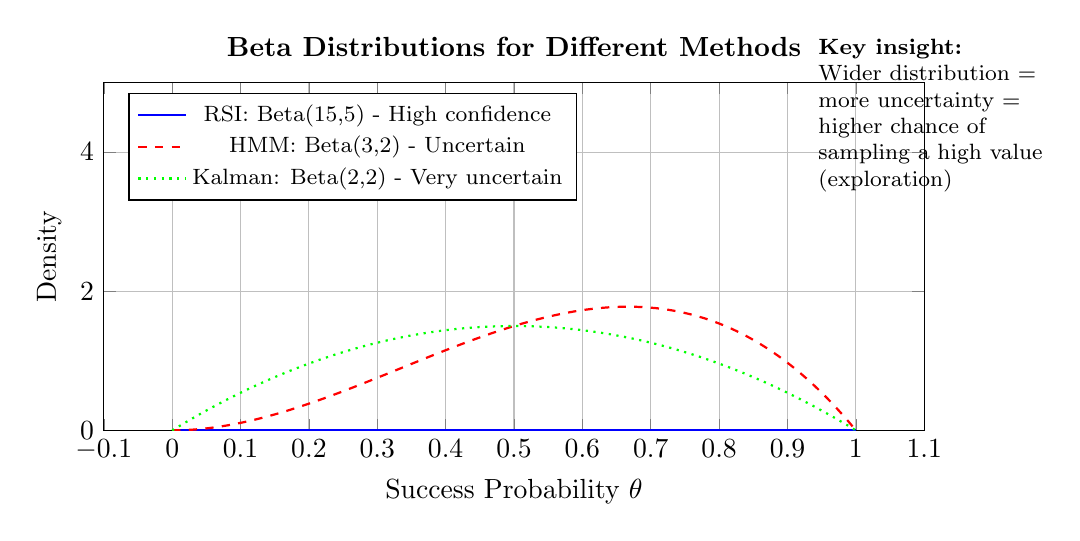
\begin{tikzpicture}
\begin{axis}[
    width=12cm, height=6cm,
    domain=0:1,
    samples=100,
    xlabel={Success Probability $\theta$},
    ylabel={Density},
    legend pos=north west,
    legend style={font=\footnotesize},
    title={\textbf{Beta Distributions for Different Methods}},
    grid=major,
    ymin=0, ymax=5
]

% Beta(15, 5) - RSI - high confidence, high success
\addplot[thick, color=blue] {(x^14)*(1-x)^4 * 2432902008176640000 / (87178291200 * 24 * 1307674368000)};
\addlegendentry{RSI: Beta(15,5) - High confidence}

% Beta(3, 2) - HMM - low confidence
\addplot[thick, color=red, dashed] {(x^2)*(1-x)^1 * 12};
\addlegendentry{HMM: Beta(3,2) - Uncertain}

% Beta(2, 2) - Kalman - uniform-ish
\addplot[thick, color=green, dotted] {(x^1)*(1-x)^1 * 6};
\addlegendentry{Kalman: Beta(2,2) - Very uncertain}

\end{axis}

% Annotation
\node[font=\footnotesize, align=left] at (10.5, 4) {
    \textbf{Key insight:}\\
    Wider distribution =\\
    more uncertainty =\\
    higher chance of\\
    sampling a high value\\
    (exploration)
};

\end{tikzpicture}
\caption{Thompson Sampling uses Beta distributions. Uncertain methods (wide distributions) may sample high values, encouraging exploration.}
\label{fig:thompson}
\end{figure}

\subsection{Enhancement 2: Contextual Baselines}

\begin{keybox}[Contextual Baseline Intuition]
A 2\% return means different things in different market conditions. In a bull market, it's average. In a bear market, it's exceptional. We need separate baselines per context.
\end{keybox}

\textbf{Context Discretization}:

We discretize market conditions into regimes:
\begin{equation}
    c = (\text{trend}, \text{volatility}, \text{regime})
\end{equation}

Example contexts:
\begin{itemize}
    \item \texttt{trend:bullish|vol:low|regime:normal}
    \item \texttt{trend:bearish|vol:high|regime:volatile}
\end{itemize}

\textbf{Per-Context Baseline}:
\begin{equation}
    \bar{R}_c = \frac{1}{n_c} \sum_{t: c_t = c} R_t
\end{equation}

\textbf{Contextual Advantage}:
\begin{equation}
    A = R - \bar{R}_c
\end{equation}

\textbf{Example}:

\begin{center}
\begin{tabular}{|l|c|c|c|}
\hline
\textbf{Context} & \textbf{Reward} & \textbf{Baseline} & \textbf{Advantage} \\
\hline
Bull market & +2\% & +2.5\% & -0.5\% (below average) \\
Bear market & +2\% & -0.5\% & +2.5\% (exceptional!) \\
\hline
\end{tabular}
\end{center}

The same reward gets different credit based on context.

% Contextual Baseline visualization
\begin{figure}[h]
\centering
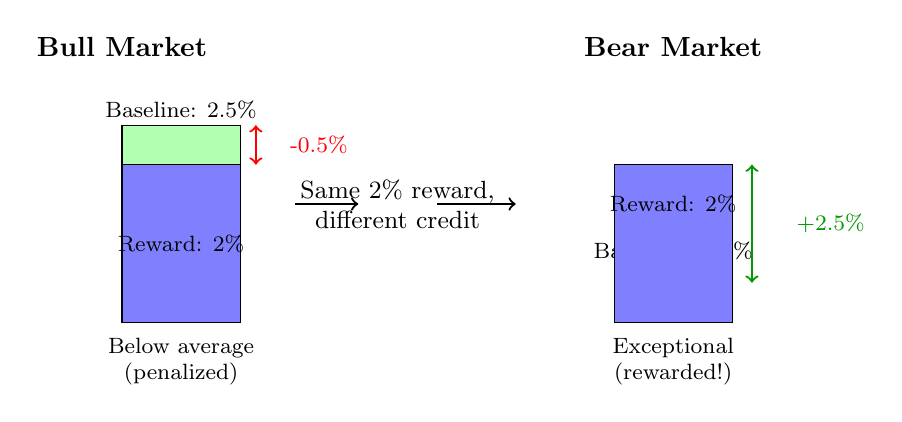
\begin{tikzpicture}[
    bar/.style={rectangle, draw, minimum width=1.5cm},
    label/.style={font=\footnotesize}
]

% Bull market scenario
\node[font=\bfseries] at (0, 3.5) {Bull Market};
\draw[fill=green!30] (0, 0) rectangle (1.5, 2.5);
\node[label] at (0.75, 2.7) {Baseline: 2.5\%};
\draw[fill=blue!50] (0, 0) rectangle (1.5, 2);
\node[label] at (0.75, 1) {Reward: 2\%};
\draw[<->, thick, red] (1.7, 2) -- (1.7, 2.5);
\node[label, red] at (2.5, 2.25) {-0.5\%};
\node[label, align=center] at (0.75, -0.5) {Below average\\(penalized)};

% Bear market scenario
\node[font=\bfseries] at (7, 3.5) {Bear Market};
\draw[fill=red!30] (6.25, 0) rectangle (7.75, 0.5);
\node[label] at (7, 0.9) {Baseline: -0.5\%};
\draw[fill=blue!50] (6.25, 0) rectangle (7.75, 2);
\node[label] at (7, 1.5) {Reward: 2\%};
\draw[<->, thick, green!60!black] (8, 0.5) -- (8, 2);
\node[label, green!60!black] at (9, 1.25) {+2.5\%};
\node[label, align=center] at (7, -0.5) {Exceptional\\(rewarded!)};

% Middle explanation
\node[font=\small, align=center] at (3.5, 1.5) {Same 2\% reward,\\different credit};
\draw[->, thick] (2.2, 1.5) -- (3, 1.5);
\draw[->, thick] (4, 1.5) -- (5, 1.5);

\end{tikzpicture}
\caption{Contextual baselines: The same 2\% return gets different credit depending on market conditions.}
\label{fig:contextual}
\end{figure}

\subsection{Enhancement 3: Multi-Step Returns}

\begin{keybox}[Multi-Step Return Intuition]
Some methods sacrifice short-term gains for long-term benefits. We need to credit methods for future outcomes, not just immediate rewards.
\end{keybox}

\textbf{$n$-Step Return}:
\begin{equation}
    G_t = R_t + \gamma R_{t+1} + \gamma^2 R_{t+2} + \ldots + \gamma^{n-1} R_{t+n-1}
\end{equation}

where $\gamma \in (0, 1)$ is the discount factor (we use $\gamma = 0.9$).

\textbf{Example}:

\begin{center}
\begin{tabular}{|l|c|c|c|c|}
\hline
\textbf{Method} & $R_0$ & $R_1$ & $R_2$ & $G$ (with $\gamma=0.9$) \\
\hline
Method A & +1\% & +0.5\% & +0.5\% & $1 + 0.45 + 0.41 = 1.86\%$ \\
Method B & -0.5\% & +3\% & +2\% & $-0.5 + 2.7 + 1.62 = 3.82\%$ \\
\hline
\end{tabular}
\end{center}

Method B looks bad initially but has better multi-step return.

% Multi-step return visualization
\begin{figure}[h]
\centering
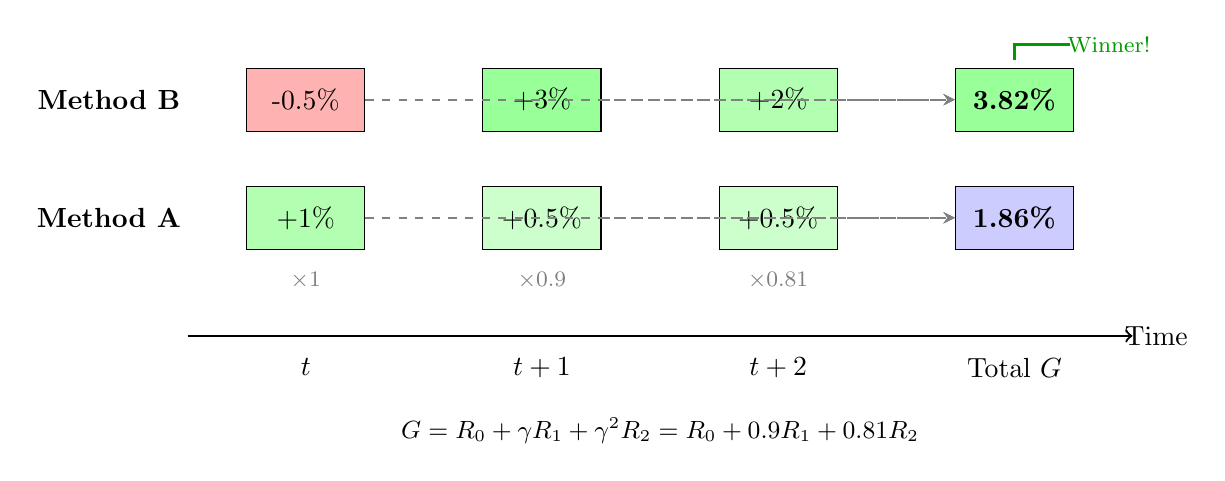
\begin{tikzpicture}[
    timestep/.style={rectangle, draw, minimum width=1.5cm, minimum height=0.8cm, align=center},
    arrow/.style={->, thick, >=stealth}
]

% Timeline
\draw[->, thick] (0, 0) -- (12, 0);
\node at (12.3, 0) {Time};

% Time labels
\node at (1.5, -0.4) {$t$};
\node at (4.5, -0.4) {$t+1$};
\node at (7.5, -0.4) {$t+2$};
\node at (10.5, -0.4) {Total $G$};

% Method A (immediate gains)
\node[timestep, fill=green!30] (a0) at (1.5, 1.5) {+1\%};
\node[timestep, fill=green!20] (a1) at (4.5, 1.5) {+0.5\%};
\node[timestep, fill=green!20] (a2) at (7.5, 1.5) {+0.5\%};
\node[timestep, fill=blue!20] (ag) at (10.5, 1.5) {\textbf{1.86\%}};
\node[font=\bfseries] at (-1, 1.5) {Method A};

% Method B (delayed gains)
\node[timestep, fill=red!30] (b0) at (1.5, 3) {-0.5\%};
\node[timestep, fill=green!40] (b1) at (4.5, 3) {+3\%};
\node[timestep, fill=green!30] (b2) at (7.5, 3) {+2\%};
\node[timestep, fill=green!40] (bg) at (10.5, 3) {\textbf{3.82\%}};
\node[font=\bfseries] at (-1, 3) {Method B};

% Discount factors
\node[font=\footnotesize, color=gray] at (1.5, 0.7) {$\times 1$};
\node[font=\footnotesize, color=gray] at (4.5, 0.7) {$\times 0.9$};
\node[font=\footnotesize, color=gray] at (7.5, 0.7) {$\times 0.81$};

% Arrows to total
\draw[arrow, dashed, gray] (a0) -- (ag);
\draw[arrow, dashed, gray] (a1) -- (ag);
\draw[arrow, dashed, gray] (a2) -- (ag);

\draw[arrow, dashed, gray] (b0) -- (bg);
\draw[arrow, dashed, gray] (b1) -- (bg);
\draw[arrow, dashed, gray] (b2) -- (bg);

% Winner indicator
\draw[thick, green!60!black] (10.5, 3.5) -- (10.5, 3.7) -- (11.2, 3.7);
\node[font=\footnotesize, green!60!black] at (11.7, 3.7) {Winner!};

% Formula
\node[font=\small] at (6, -1.2) {$G = R_0 + \gamma R_1 + \gamma^2 R_2 = R_0 + 0.9 R_1 + 0.81 R_2$};

\end{tikzpicture}
\caption{Multi-step returns with $\gamma = 0.9$. Method B has worse immediate reward but better total return.}
\label{fig:multistep}
\end{figure}

%==============================================================================
\section{Population-Based Learning}
%==============================================================================

\subsection{Population Structure}

\begin{center}
\begin{tabular}{|l|c|l|}
\hline
\textbf{Role} & \textbf{Population Size} & \textbf{What Varies} \\
\hline
Analyst & 5 agents & Method selections, preferences \\
Researcher & 5 agents & Method selections, preferences \\
Trader & 5 agents & Method selections, preferences \\
Risk Manager & 5 agents & Method selections, preferences \\
\hline
\textbf{Total} & 20 agents & \\
\hline
\end{tabular}
\end{center}

% Population structure visualization
\begin{figure}[h]
\centering
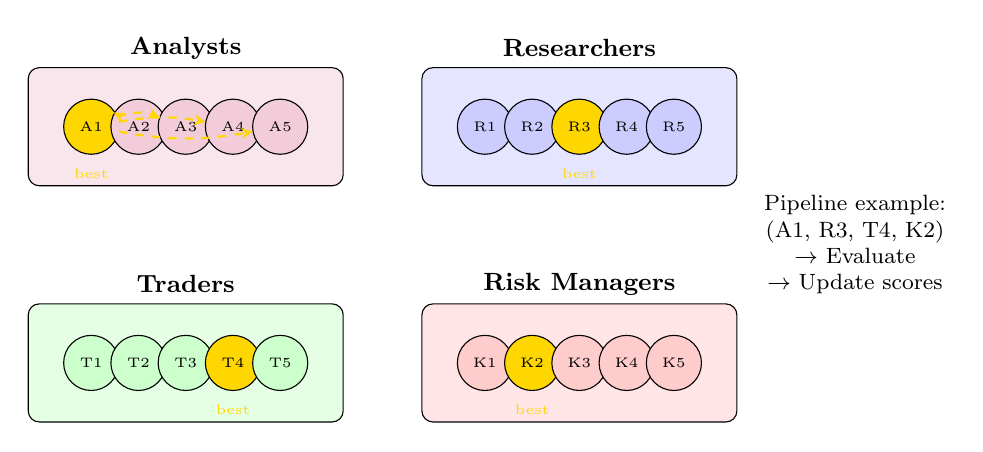
\begin{tikzpicture}[
    agent/.style={circle, draw, minimum size=0.7cm, font=\tiny},
    best/.style={circle, draw, fill=gold, minimum size=0.7cm, font=\tiny},
    pop/.style={rectangle, draw, rounded corners, minimum width=4cm, minimum height=1.5cm},
    arrow/.style={->, thick, >=stealth, dashed}
]

% Analyst population
\node[pop, fill=purple!10] (apop) at (0, 0) {};
\node[font=\small\bfseries] at (0, 1) {Analysts};
\node[best] (a1) at (-1.2, 0) {A1};
\node[agent, fill=purple!20] (a2) at (-0.6, 0) {A2};
\node[agent, fill=purple!20] (a3) at (0, 0) {A3};
\node[agent, fill=purple!20] (a4) at (0.6, 0) {A4};
\node[agent, fill=purple!20] (a5) at (1.2, 0) {A5};
\node[font=\tiny, color=gold] at (-1.2, -0.6) {best};

% Researcher population
\node[pop, fill=blue!10] (rpop) at (5, 0) {};
\node[font=\small\bfseries] at (5, 1) {Researchers};
\node[agent, fill=blue!20] (r1) at (3.8, 0) {R1};
\node[agent, fill=blue!20] (r2) at (4.4, 0) {R2};
\node[best] (r3) at (5, 0) {R3};
\node[agent, fill=blue!20] (r4) at (5.6, 0) {R4};
\node[agent, fill=blue!20] (r5) at (6.2, 0) {R5};
\node[font=\tiny, color=gold] at (5, -0.6) {best};

% Trader population
\node[pop, fill=green!10] (tpop) at (0, -3) {};
\node[font=\small\bfseries] at (0, -2) {Traders};
\node[agent, fill=green!20] (t1) at (-1.2, -3) {T1};
\node[agent, fill=green!20] (t2) at (-0.6, -3) {T2};
\node[agent, fill=green!20] (t3) at (0, -3) {T3};
\node[best] (t4) at (0.6, -3) {T4};
\node[agent, fill=green!20] (t5) at (1.2, -3) {T5};
\node[font=\tiny, color=gold] at (0.6, -3.6) {best};

% Risk population
\node[pop, fill=red!10] (kpop) at (5, -3) {};
\node[font=\small\bfseries] at (5, -2) {Risk Managers};
\node[agent, fill=red!20] (k1) at (3.8, -3) {K1};
\node[best] (k2) at (4.4, -3) {K2};
\node[agent, fill=red!20] (k3) at (5, -3) {K3};
\node[agent, fill=red!20] (k4) at (5.6, -3) {K4};
\node[agent, fill=red!20] (k5) at (6.2, -3) {K5};
\node[font=\tiny, color=gold] at (4.4, -3.6) {best};

% Knowledge transfer arrows
\draw[arrow, color=gold] (a1) to[bend left=30] (a2);
\draw[arrow, color=gold] (a1) to[bend left=20] (a3);
\draw[arrow, color=gold] (a1) to[bend left=10] (a4);
\draw[arrow, color=gold] (a1) to[bend right=10] (a5);

% Pipeline example
\node[font=\footnotesize, align=center] at (8.5, -1.5) {Pipeline example:\\(A1, R3, T4, K2)\\$\rightarrow$ Evaluate\\$\rightarrow$ Update scores};

\end{tikzpicture}
\caption{Population structure: 4 roles $\times$ 5 agents = 20 agents. Gold = best performer, transfers knowledge to others.}
\label{fig:population}
\end{figure}

\subsection{Pipeline Combinations}

In each iteration, we sample \textbf{pipeline combinations}:
\begin{equation}
    \text{Pipeline} = (\text{Analyst}_i, \text{Researcher}_j, \text{Trader}_k, \text{Risk}_l)
\end{equation}

With 5 agents per role: $5^4 = 625$ possible pipelines.

We sample 25 pipelines per iteration to keep computation tractable.

\subsection{Knowledge Transfer}

Every 10 iterations, we transfer knowledge from best to others:

\begin{algorithm}
\caption{Knowledge Transfer}
\begin{algorithmic}[1]
\FOR{each role $r \in \{\text{Analyst}, \text{Researcher}, \text{Trader}, \text{Risk}\}$}
    \STATE $a^* \leftarrow$ best agent in role $r$ (by average reward)
    \FOR{each agent $a \in$ role $r$, $a \neq a^*$}
        \STATE $\pi^a \leftarrow (1 - \tau) \cdot \pi^a + \tau \cdot \pi^{a^*}$ \COMMENT{Soft preference update}
        \STATE $\alpha^a \leftarrow (1 - \tau) \cdot \alpha^a + \tau \cdot \alpha^{a^*}$ \COMMENT{Thompson params}
    \ENDFOR
\ENDFOR
\end{algorithmic}
\end{algorithm}

Where $\tau = 0.1$ (transfer rate).

\textbf{Key insight}: We transfer \textit{preferences} (meta-knowledge about what works), not parameters of the methods themselves.

\subsection{Diversity Preservation}

To prevent population collapse (all agents converging to same methods):

\begin{enumerate}
    \item \textbf{Measure diversity}: Jaccard distance between agent selections
    \begin{equation}
        D = \frac{1}{\binom{N}{2}} \sum_{i < j} \left(1 - \frac{|S^i \cap S^j|}{|S^i \cup S^j|}\right)
    \end{equation}

    \item \textbf{If diversity $< 0.3$}: Boost exploration rate for non-best agents

    \item \textbf{Result}: Population maintains variety while still learning from best
\end{enumerate}

%==============================================================================
\section{Data Pipeline}
%==============================================================================

\subsection{Price Data}

\textbf{Source}: Bybit perpetual futures (4-hour candles)

\textbf{Assets}: 5 cryptocurrencies

\begin{center}
\begin{tabular}{|l|l|l|}
\hline
\textbf{Symbol} & \textbf{Name} & \textbf{Role} \\
\hline
BTC & Bitcoin & Primary benchmark \\
ETH & Ethereum & Smart contract platform \\
SOL & Solana & High-performance L1 \\
DOGE & Dogecoin & Retail sentiment indicator \\
XRP & Ripple & Payment-focused \\
\hline
\end{tabular}
\end{center}

\textbf{Features per asset}: OHLCV + Open Interest + Funding Rate + Long/Short Ratio

\subsection{Cross-Asset Features}

We compute 8 market-wide signals:

\begin{enumerate}
    \item \textbf{BTC Dominance}: BTC market cap relative to total
    \item \textbf{Altcoin Momentum}: Average momentum of non-BTC assets
    \item \textbf{ETH/BTC Ratio}: Risk-on/risk-off indicator
    \item \textbf{Cross OI Delta}: Aggregate open interest changes
    \item \textbf{Aggregate Funding}: Market-wide funding rate
    \item \textbf{Risk-On/Risk-Off}: Composite sentiment
    \item \textbf{Market Volatility}: Aggregate volatility measure
    \item \textbf{Cross-Correlation}: Asset correlation dynamics
\end{enumerate}

\subsection{News Pipeline}

\textbf{Source}: Bocha AI web search API

\textbf{Process}:
\begin{enumerate}
    \item Generate asset-specific queries (macro + micro news)
    \item Search via Bocha API
    \item Score source credibility (tier system)
    \item Enrich with LLM (sentiment, entities, impact)
    \item Aggregate into market digest
\end{enumerate}

%==============================================================================
\section{Project Structure}
%==============================================================================

\begin{lstlisting}[basicstyle=\ttfamily\footnotesize]
trading_agents/
|-- population/                # Core innovation
|   |-- selector.py           # MethodSelector class
|   |-- inventories.py        # 47 methods across 4 roles
|   |-- selector_workflow.py  # Learning loop
|   |-- transfer.py           # Knowledge transfer strategies
|   `-- scoring.py            # Shapley-based credit assignment
|
|-- backtesting/              # Backtesting engine
|   |-- engine.py             # BacktestEngine + run_population_backtest
|   `-- executor.py           # Order execution simulation
|
|-- services/                 # Infrastructure
|   |-- experiment_logger.py  # Structured JSONL logging
|   |-- scheduler.py          # 4-hour paper trading scheduler
|   |-- neurips_export.py     # Publication figure generation
|   |-- llm.py                # LLM integration
|   `-- bybit_client.py       # Exchange API
|
|-- api/                      # Dashboard backend
|   `-- server.py             # FastAPI + WebSocket server
|
|-- agents/                   # Agent implementations
|   |-- analyst.py, researcher.py, trader.py, risk.py
|   `-- admin.py              # Monitoring/reporting
|
`-- config/                   # Configuration

dashboard/                    # React Visualization Dashboard
|-- src/components/           # AgentPopulation, MethodHeatmap, etc.
`-- src/app/                  # Next.js app with dark theme

tests/                        # Test suite
|-- conftest.py               # Pytest fixtures with mock data
`-- test_*.py                 # Workflow, selection, transfer tests
\end{lstlisting}

%==============================================================================
\section{Anticipated Questions and Answers}
%==============================================================================

\begin{questionbox}[Q1: Why not use Deep RL (PPO, SAC)?]
\textbf{Answer}: Deep RL requires 100K+ samples, is prone to instability, and produces uninterpretable policies. Our bandit-based approach achieves competitive performance with 100$\times$ fewer samples while remaining fully interpretable. In finance, interpretability and sample efficiency are critical---traders need to understand why the system makes decisions.
\end{questionbox}

\begin{questionbox}[Q2: Why 5 agents per role? Why not more/fewer?]
\textbf{Answer}: 5 provides enough diversity for meaningful exploration while keeping computation tractable ($5^4 = 625$ pipeline combinations). Fewer agents risk premature convergence; more agents increase computational cost without proportional benefit due to diminishing returns.
\end{questionbox}

\begin{questionbox}[Q3: How do you handle the credit assignment problem?]
\textbf{Answer}: We use three approaches:
\begin{enumerate}
    \item \textbf{Individual scoring}: Each agent scored by average reward when participating
    \item \textbf{Pipeline scoring}: Consider how agents work together
    \item \textbf{Shapley values}: Fair credit attribution from cooperative game theory
\end{enumerate}
\end{questionbox}

\begin{questionbox}[Q4: What prevents all agents from converging to the same methods?]
\textbf{Answer}: Diversity preservation. We measure selection diversity via Jaccard distance. If diversity drops below 0.3, we boost exploration rates for non-best agents. Thompson Sampling also naturally maintains exploration through uncertainty.
\end{questionbox}

\begin{questionbox}[Q5: How does this compare to AutoML?]
\textbf{Answer}: Similar spirit but different focus. AutoML typically selects model architectures and hyperparameters once before training. We continuously adapt method selection during trading based on ongoing performance. It's more like online AutoML with population-based exploration.
\end{questionbox}

\begin{questionbox}[Q6: Can this overfit to recent market conditions?]
\textbf{Answer}: We mitigate overfitting through:
\begin{enumerate}
    \item \textbf{Contextual baselines}: Methods are evaluated relative to market regime
    \item \textbf{Population diversity}: Multiple agents prevent convergence to single strategy
    \item \textbf{Soft updates} ($\tau = 0.1$): Gradual preference transfer, not hard copying
    \item \textbf{Thompson Sampling}: Maintains exploration even as preferences develop
\end{enumerate}
\end{questionbox}

\begin{questionbox}[Q7: What's the computational cost?]
\textbf{Answer}: Very low compared to deep RL:
\begin{itemize}
    \item No neural network training
    \item Main cost is evaluating 25 pipelines per iteration
    \item Each pipeline: feature computation + forecast + order generation
    \item Runs on CPU, no GPU required
\end{itemize}
\end{questionbox}

\begin{questionbox}[Q8: How do you evaluate this system?]
\textbf{Answer}: Multiple metrics:
\begin{itemize}
    \item \textbf{Sharpe Ratio}: Risk-adjusted returns
    \item \textbf{Maximum Drawdown}: Worst peak-to-trough loss
    \item \textbf{Hit Rate}: Percentage of profitable trades
    \item \textbf{Calibration ECE}: Uncertainty quality
    \item \textbf{Learning curves}: Do preferences converge? Does performance improve?
\end{itemize}
\end{questionbox}

%==============================================================================
\section{Complete Learning Loop}
%==============================================================================

\begin{figure}[h]
\centering
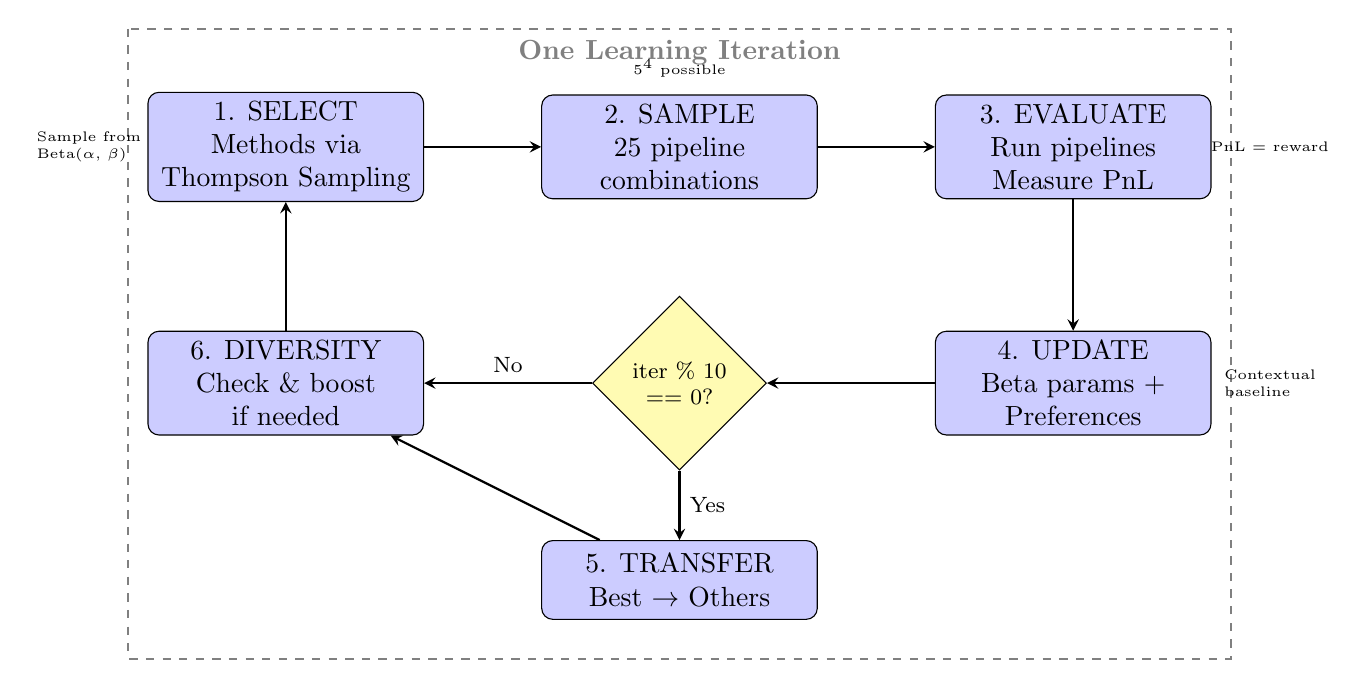
\begin{tikzpicture}[
    loopstep/.style={rectangle, draw, rounded corners, fill=blue!20, minimum width=3.5cm, minimum height=1cm, align=center},
    decision/.style={diamond, draw, fill=yellow!30, minimum width=2cm, minimum height=1.5cm, align=center, font=\footnotesize},
    arrow/.style={->, thick, >=stealth}
]

% Main loop
\node[loopstep] (select) at (0, 0) {1. SELECT\\Methods via\\Thompson Sampling};
\node[loopstep] (pipeline) at (5, 0) {2. SAMPLE\\25 pipeline\\combinations};
\node[loopstep] (evaluate) at (10, 0) {3. EVALUATE\\Run pipelines\\Measure PnL};

\node[loopstep] (update) at (10, -3) {4. UPDATE\\Beta params +\\Preferences};
\node[decision] (check) at (5, -3) {iter \% 10\\== 0?};
\node[loopstep] (transfer) at (5, -5.5) {5. TRANSFER\\Best $\rightarrow$ Others};
\node[loopstep] (diversity) at (0, -3) {6. DIVERSITY\\Check \& boost\\if needed};

% Arrows
\draw[arrow] (select) -- (pipeline);
\draw[arrow] (pipeline) -- (evaluate);
\draw[arrow] (evaluate) -- (update);
\draw[arrow] (update) -- (check);
\draw[arrow] (check) -- node[right, font=\footnotesize] {Yes} (transfer);
\draw[arrow] (check) -- node[above, font=\footnotesize] {No} (diversity);
\draw[arrow] (transfer) -- (diversity);
\draw[arrow] (diversity) -- (select);

% Iteration label
\draw[dashed, gray, thick] (-2, 1.5) rectangle (12, -6.5);
\node[font=\bfseries, gray] at (5, 1.2) {One Learning Iteration};

% Side annotations
\node[font=\tiny, align=left] at (-2.5, 0) {Sample from\\Beta($\alpha$, $\beta$)};
\node[font=\tiny, align=left] at (5, 1) {$5^4$ possible};
\node[font=\tiny, align=left] at (12.5, 0) {PnL = reward};
\node[font=\tiny, align=left] at (12.5, -3) {Contextual\\baseline};

\end{tikzpicture}
\caption{Complete learning loop for one iteration. Steps repeat, with knowledge transfer every 10 iterations.}
\label{fig:loop}
\end{figure}

%==============================================================================
\section{Key Takeaways}
%==============================================================================

% Visual summary
\begin{figure}[h]
\centering
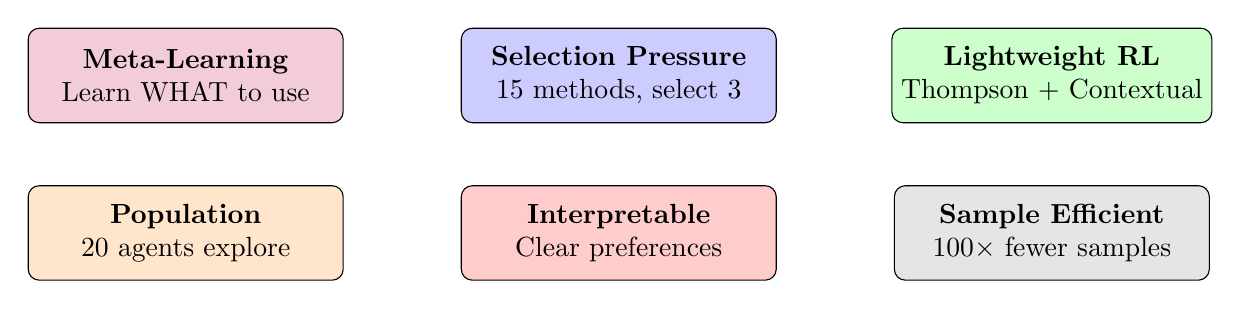
\begin{tikzpicture}[
    box/.style={rectangle, draw, rounded corners, fill=#1, minimum width=4cm, minimum height=1.2cm, align=center},
]

\node[box=purple!20] at (0, 0) {\textbf{Meta-Learning}\\Learn WHAT to use};
\node[box=blue!20] at (5.5, 0) {\textbf{Selection Pressure}\\15 methods, select 3};
\node[box=green!20] at (11, 0) {\textbf{Lightweight RL}\\Thompson + Contextual};

\node[box=orange!20] at (0, -2) {\textbf{Population}\\20 agents explore};
\node[box=red!20] at (5.5, -2) {\textbf{Interpretable}\\Clear preferences};
\node[box=gray!20] at (11, -2) {\textbf{Sample Efficient}\\100$\times$ fewer samples};

\end{tikzpicture}
\caption{Six key properties of PopAgent.}
\label{fig:takeaways}
\end{figure}

\begin{enumerate}
    \item \textbf{Method Selection as Meta-Learning}: Agents learn WHAT to use, not just parameters

    \item \textbf{Selection Pressure}: Inventory (15) $>$ Selection (3) creates meaningful choices

    \item \textbf{Lightweight RL}: Thompson Sampling + Contextual Baselines + Multi-Step Returns

    \item \textbf{Population Dynamics}: 20 agents explore, best knowledge transfers to others

    \item \textbf{Interpretability}: Clear preferences, no black-box neural networks

    \item \textbf{Sample Efficiency}: Works with limited financial data
\end{enumerate}

%==============================================================================
\section{Practical Usage}
%==============================================================================

\subsection{How to Run the System}

\begin{lstlisting}[language=bash]
# 1. Setup environment
python -m venv .venv
source .venv/bin/activate
pip install -e .

# 2. Copy price data
cp /path/to/Bybit_CSV_Data/*.csv data/bybit/

# 3. Set API keys (in .env file)
BOCHA_API_KEY=your_news_api_key
BYBIT_TESTNET_KEY=your_testnet_key
BYBIT_TESTNET_SECRET=your_testnet_secret

# 4. Run the adaptive method selection workflow
python -m trading_agents.cli selector --iterations 50
\end{lstlisting}

\subsection{Expected Output}

After running, you'll see:
\begin{itemize}
    \item \textbf{Method preferences}: Which methods each agent prefers
    \item \textbf{Performance metrics}: Sharpe ratio, PnL, drawdown
    \item \textbf{Learning curves}: How preferences evolved over iterations
    \item \textbf{Best pipeline}: Top-performing agent combination
\end{itemize}

\subsection{Running the Visualization Dashboard}

PopAgent includes a modern React dashboard for visualizing the learning process:

\begin{lstlisting}[language=bash]
# 1. Start the backend API server
python -m trading_agents.cli api --port 8000

# 2. In a separate terminal, start the React dashboard
cd dashboard
npm install
npm run dev

# 3. Open http://localhost:3000 in your browser
\end{lstlisting}

The dashboard provides:
\begin{itemize}
    \item \textbf{Population View}: Grid visualization of all 20 agents across 4 roles
    \item \textbf{Method Heatmap}: Selection frequency per agent/method
    \item \textbf{Learning Timeline}: PnL over iterations with transfer markers
    \item \textbf{Pipeline Flow}: Animated visualization of data through agents
    \item \textbf{Reasoning Panel}: LLM explanations for method selection
    \item \textbf{Knowledge Transfer}: Timeline of preference transfers
\end{itemize}

\subsection{Running Population Backtest}

Test the PopAgent system on historical data:

\begin{lstlisting}[language=bash]
# Run backtest on BTC data
python -m trading_agents.cli backtest --symbol BTC --population-size 5

# Specify date range
python -m trading_agents.cli backtest --symbol ETH \
    --start 2024-01-01 --end 2024-06-01

# With custom capital
python -m trading_agents.cli backtest --symbol BTC --capital 50000
\end{lstlisting}

\subsection{Exporting for NeurIPS Paper}

Generate publication-ready figures and tables:

\begin{lstlisting}[language=bash]
# Export all figures and tables
python -m trading_agents.cli export \
    --experiment-id backtest_BTC_20241220_143022 \
    --output-dir exports/neurips \
    --format pdf latex

# Generated files:
# - figure1_learning_curve.pdf
# - figure2_method_popularity.pdf
# - figure3_cumulative_returns.pdf
# - figure4_diversity.pdf
# - table1_performance.tex
# - table2_methods.tex
# - appendix_reasoning_traces.json
\end{lstlisting}

\subsection{Configuration}

Key settings in \texttt{configs/multi\_asset.yaml}:

\begin{lstlisting}[language=yaml]
population:
  size: 5               # Agents per role
  max_methods: 3        # Methods selected per agent
  transfer_frequency: 10  # Transfer every N iterations
  learning_rate: 0.1    # Preference update rate
  exploration_rate: 0.15  # Random exploration
\end{lstlisting}

%==============================================================================
\section{References for Further Reading}
%==============================================================================

\begin{itemize}
    \item \textbf{Thompson Sampling}: Thompson (1933), ``On the likelihood that one unknown probability exceeds another''
    \item \textbf{Population-Based Training}: Jaderberg et al. (2017), ``Population Based Training of Neural Networks''
    \item \textbf{Shapley Values}: Shapley (1953), ``A value for n-person games''
    \item \textbf{Contextual Bandits}: Li et al. (2010), ``A Contextual-Bandit Approach to Personalized News Article Recommendation''
\end{itemize}

%==============================================================================
\appendix
\section{Full System Architecture Diagram}
%==============================================================================

\begin{figure}[h]
\centering
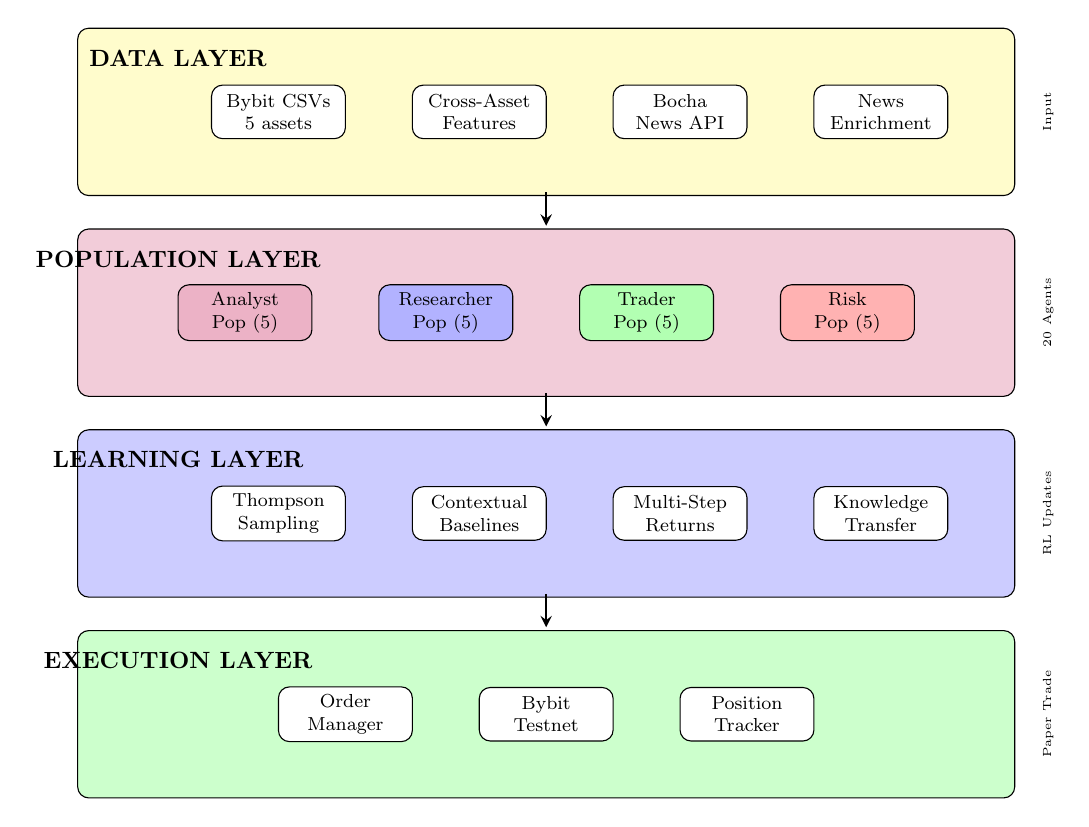
\begin{tikzpicture}[scale=0.85, transform shape,
    layer/.style={rectangle, draw, rounded corners, minimum width=14cm, minimum height=2.5cm, fill=#1},
    component/.style={rectangle, draw, rounded corners, fill=white, minimum width=2cm, minimum height=0.8cm, font=\footnotesize, align=center},
    arrow/.style={->, thick, >=stealth}
]

% Layer 1: Data Input
\node[layer=yellow!20] (data) at (0, 8) {};
\node[font=\bfseries] at (-5.5, 8.8) {DATA LAYER};
\node[component] at (-4, 8) {Bybit CSVs\\5 assets};
\node[component] at (-1, 8) {Cross-Asset\\Features};
\node[component] at (2, 8) {Bocha\\News API};
\node[component] at (5, 8) {News\\Enrichment};

% Layer 2: Population
\node[layer=purple!20] (pop) at (0, 5) {};
\node[font=\bfseries] at (-5.5, 5.8) {POPULATION LAYER};
\node[component, fill=purple!30] at (-4.5, 5) {Analyst\\Pop (5)};
\node[component, fill=blue!30] at (-1.5, 5) {Researcher\\Pop (5)};
\node[component, fill=green!30] at (1.5, 5) {Trader\\Pop (5)};
\node[component, fill=red!30] at (4.5, 5) {Risk\\Pop (5)};

% Layer 3: Learning
\node[layer=blue!20] (learn) at (0, 2) {};
\node[font=\bfseries] at (-5.5, 2.8) {LEARNING LAYER};
\node[component] at (-4, 2) {Thompson\\Sampling};
\node[component] at (-1, 2) {Contextual\\Baselines};
\node[component] at (2, 2) {Multi-Step\\Returns};
\node[component] at (5, 2) {Knowledge\\Transfer};

% Layer 4: Execution
\node[layer=green!20] (exec) at (0, -1) {};
\node[font=\bfseries] at (-5.5, -0.2) {EXECUTION LAYER};
\node[component] at (-3, -1) {Order\\Manager};
\node[component] at (0, -1) {Bybit\\Testnet};
\node[component] at (3, -1) {Position\\Tracker};

% Arrows between layers
\draw[arrow] (0, 6.8) -- (0, 6.3);
\draw[arrow] (0, 3.8) -- (0, 3.3);
\draw[arrow] (0, 0.8) -- (0, 0.3);

% Side labels
\node[font=\tiny, rotate=90] at (7.5, 8) {Input};
\node[font=\tiny, rotate=90] at (7.5, 5) {20 Agents};
\node[font=\tiny, rotate=90] at (7.5, 2) {RL Updates};
\node[font=\tiny, rotate=90] at (7.5, -1) {Paper Trade};

\end{tikzpicture}
\caption{Complete system architecture showing the four main layers.}
\label{fig:architecture}
\end{figure}

%==============================================================================
\section{Method Inventory Reference}
%==============================================================================

\begin{table}[h]
\centering
\footnotesize
\caption{Complete method inventories for all four agent roles.}
\begin{tabular}{|l|l|p{8cm}|}
\hline
\textbf{Role} & \textbf{Category} & \textbf{Methods} \\
\hline
\multirow{4}{*}{Analyst (15)}
& Technical & RSI, MACD, BollingerBands, ADX, Stochastic \\
& Statistical & Autocorrelation, VolatilityClustering, MeanReversion, Cointegration \\
& Decomposition & STL, WaveletTransform, FourierAnalysis \\
& ML & HMM\_Regime, KalmanFilter, IsolationForest \\
\hline
\multirow{3}{*}{Researcher (12)}
& Statistical & ARIMA, ExponentialSmoothing, VAR, GARCH \\
& ML & RandomForest, GradientBoosting, LSTM, TemporalFusion \\
& Uncertainty & Bootstrap, QuantileRegression, Bayesian, ConformalPrediction \\
\hline
\multirow{3}{*}{Trader (10)}
& Execution & AggressiveMarket, PassiveLimit, TWAP, VWAP \\
& Sizing & KellyCriterion, FixedFractional, VolatilityScaled \\
& Entry & MomentumEntry, ContrarianEntry, BreakoutEntry \\
\hline
\multirow{4}{*}{Risk (10)}
& Position & MaxLeverage, MaxPositionSize, ConcentrationLimit \\
& Loss & MaxDrawdown, DailyStopLoss, TrailingStop \\
& Metrics & VaR, ExpectedShortfall \\
& Dynamic & VolatilityAdjusted, RegimeAware \\
\hline
\end{tabular}
\label{tab:full_inventory}
\end{table}

%==============================================================================
\section{Notation Summary}
%==============================================================================

\begin{table}[h]
\centering
\caption{Mathematical notation used throughout this document.}
\begin{tabular}{|l|l|}
\hline
\textbf{Symbol} & \textbf{Meaning} \\
\hline
$\mathcal{M}$ & Method inventory (set of available methods) \\
$|\mathcal{M}|$ & Inventory size (e.g., 15 for Analyst) \\
$S$ & Selected methods (subset of $\mathcal{M}$, typically $|S|=3$) \\
$k$ & Number of methods to select \\
$\alpha_m, \beta_m$ & Beta distribution parameters for method $m$ \\
$\theta_m$ & Sampled success probability for method $m$ \\
$\pi$ & Preference vector over methods \\
$\bar{R}_c$ & Baseline reward for context $c$ \\
$A$ & Advantage (reward minus baseline) \\
$\gamma$ & Discount factor for multi-step returns (default 0.9) \\
$G_t$ & Multi-step return starting at time $t$ \\
$\tau$ & Transfer rate for knowledge sharing (default 0.1) \\
$D$ & Selection diversity (Jaccard distance) \\
$N$ & Population size (default 5 agents per role) \\
\hline
\end{tabular}
\label{tab:notation}
\end{table}

\end{document}
